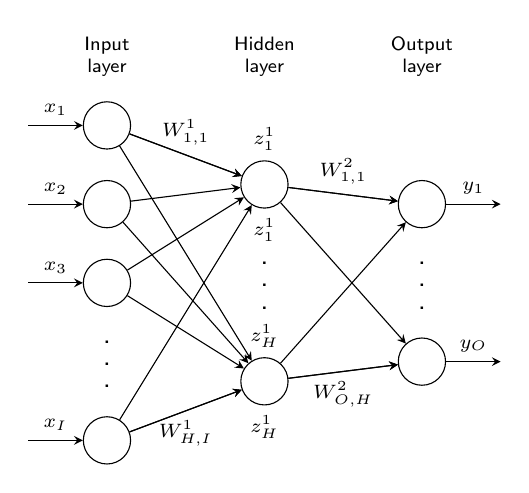
\begin{tikzpicture}[x=1.0cm, y=1.0cm, >=stealth, font=\sffamily\scriptsize]
    \tikzstyle{every neuron}=[circle, draw, minimum size=.6cm]
    \tikzstyle{neuron missing}=[draw=none, scale=2, text height=0.333cm, execute at begin node={\color{black}\tiny$\vdots$}]
    
    % Inputs nodes
    \foreach \m/\l [count=\y] in {1,2,3,missing,4}
      \node [every neuron/.try, neuron \m/.try] (input-\m) at (0,2.5-\y) {};
      
    % Hidden nodes
    \foreach \m [count=\y] in {1,missing,2} {
        \node [every neuron/.try, neuron \m/.try ] (hidden-\m) at (2,2-\y*1.25) {};
    }
        % \ifthenelse{\y=2}
        %     {\node [every neuron/.try, neuron \m/.try ] (hidden-\m) at (2,2-\y*1.25) {};}
        %     {\node [every neuron/.try, neuron \m/.try ] (hidden-\m) at (2,2-\y*1.25) {$a_\m^\bra{0}$};}
        % }
      %\node [every neuron/.try, neuron \m/.try ] (hidden-\m) at (2,2-\y*1.25) {$a_\m^\bra{0}$};
      
    % Outputs nodes
    \foreach \m [count=\y] in {1,missing,2}
      \node [every neuron/.try, neuron \m/.try ] (output-\m) at (4,1.5-\y) {};
      
    % Names on inputs
    \foreach \l [count=\i] in {1,2,3,I}
      \draw [<-] (input-\i) -- ++(-1,0)
        node [above, midway] {$x_\l$};
        
    % Names on hidden
    \foreach \l [count=\i] in {1,H} {
        \ifthenelse{\i=1}
            {\node [above] at (hidden-\i.north) {$z^\bra{1}_\l$};}
            {\node [below] at (hidden-\i.south) {$z^\bra{1}_\l$};}
    }
      
    % Names on outputs
    \foreach \l [count=\i] in {1,O}
      \draw [->] (output-\i) -- ++(1,0)
        node [above, midway] {$y_\l$};
        
    % Inputs -> Hidden
    \foreach \i in {1,...,4} {
      \foreach \j in {1,...,2} {
        %\draw [->] (input-\i) -- (hidden-\j);
        \ifthenelse{\i=1 \AND \j=1 \OR \i=4 \AND \j=2}
            {}
            {\draw [->] (input-\i) -- (hidden-\j);}
        }
    }
    \draw [->] (input-1) --node[above]{$W^{\bra{1}}_{1,1}$} (hidden-1);
    \draw [->] (input-4) --node[below]{$W^{\bra{1}}_{H,I}$} (hidden-2);
        
    % Hidden -> Outputs
    \foreach \i in {1,...,2}  {
      \foreach \j in {1,...,2} {
        % \draw [->] (hidden-\i) -- (output-\j);
        \ifthenelse{\i=1 \AND \j=1 \OR \i=2 \AND \j=2}
            {}
            {\draw [->] (hidden-\i) -- (output-\j);}
        }
    }
    \draw [->] (hidden-1) --node[above]{$W^{\bra{2}}_{1,1}$} (output-1);
    \draw [->] (hidden-2) --node[below]{$W^{\bra{2}}_{O,H}$} (output-2);
    
    % Layer names
    \foreach \l [count=\x from 0] in {Input, Hidden, Output}
      \node [align=center, above] at (\x*2,2) {\l \\ layer};
\end{tikzpicture}